\hypertarget{portfolio}{%
\section{Portfólió}\label{portfolio}}

A tanulási-tanítási egységek, a modulok eredményeiből, a produktumokból
és visszajelzésekből a gyerek és a mentor portfóliót állít össze, hogy a
tanulás mintázatait észlelhesse, és a tanárok tudatosabban tudják a
gyereket segíteni a céljai kitalálásában és elérésében. A portfólió a
gyerek eredményeinek nyomon követését is szolgálja, és egyúttal a szülők
felé történő visszajelzés eszköze is. Minden gyerek portfóliója
folyamatosan épül: tartalmazza az általa elvégzett feladatokat,
projekteket vagy azok dokumentációját, alkotásait, eredményeit, az
esetleges vizsgák eredményeit és a társaitól, tanáraitól kapott
visszajelzéseket. A \emph{portfólió célja}, hogy minden információ
meglegyen ahhoz, hogy

\begin{itemize}
\tightlist
\item
  a gyerek és mentora fel tudja mérni, hogy sikerült-e a kitűzött
  célokat elérni, illetve mire van szüksége még a gyereknek új célok
  eléréséhez;
\item
  a szülő folyamatosan rálásson a gyereke tanulási útjára;
\item
  megítélhető legyen, hogy a tantárgyi követelményekhez képest hol tart
  a gyerek;
\item
  a gyerek a portfólió megtekintésével visszaemlékezhessen a tanultakra,
  ismételhessen, tudása elmélyülhessen;
\item
  eredményei alapján bizonyítványt lehessen kiállítani.
\end{itemize}

\begin{figure}
\centering
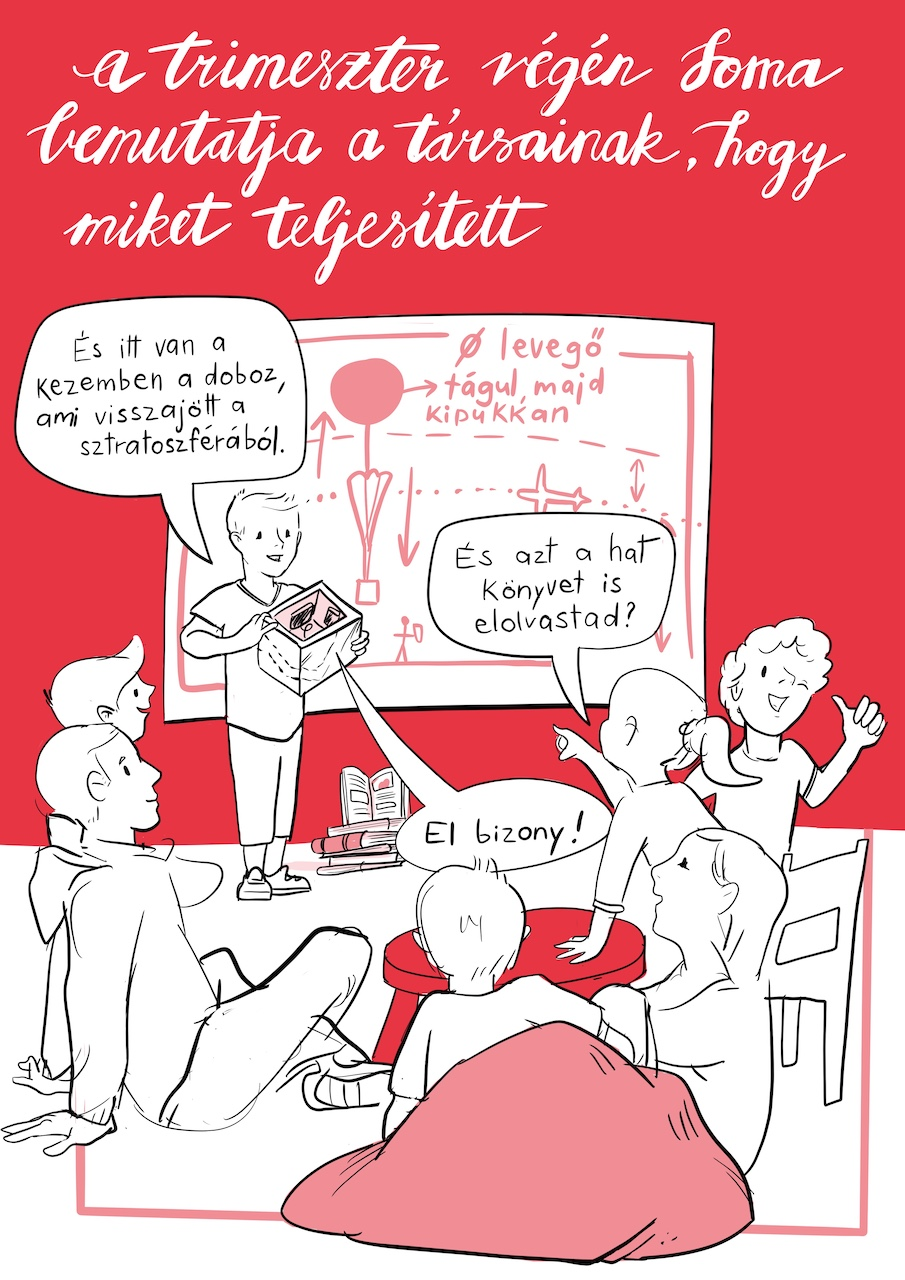
\includegraphics{pics/4a_portfolio_soma.jpg}
\caption{Portfólió  tartalmazza a gyerek által elvégzett feladatokat,
projekteket, alkotásait.}
\end{figure}

A portfólió folyamatosan frissül, a mindennapi, formális, nem-for\-má\-lis
és informális tanulási helyzetek bármikor adhatnak okot a portfólió
frissítésére. Az iskola életében kiemelt szerepe van a következő
eseményeknek.

Minden \emph{modul végeztével} a portfólióba kerül:

\begin{enumerate}
\def\labelenumi{\arabic{enumi}.}
\tightlist
\item
  A képesség elsajátításának, tanulási eredmény elérésének a ténye. Ha a
  modul során a gyerek megtanult százas számkörben alapműveleteket
  végezni, akkor annyi kerül be a portfólióba, hogy „\emph{Szóban és
  írásban összead, kivon, szoroz és oszt a százas számkörben}''.
  Amennyiben a készséget-képességet a gyerek és a tanár megítélése
  alapján nem sikerült megfelelően elsajátítani, úgy a gyakorlás ténye
  kerül be a portfólióba.
\item
  Az alkotás vagy a projektmunka eredménye, ha a modul célja egy alkotás
  létrehozása volt.
\item
  A részvétel ténye, ha a jelenlét volt a modul célja (például
  kirándulás az Országos Kéktúra útvonalán).
\item
  Az elvégzett vizsgák, tudáspróbák, képességfelmérők, diagnózisok
  eredményei tanulási eredmények igazolásával is járnak.
\item
  A \emph{kipakolás} célja, hogy a gyerekek a tanároknak, szülőknek és
  más érintetteknek bemutassák elvégzett munkájukat, azaz a
  portfólióváltozásukat. A kipakolásra való felkészülés tulajdonképpen a
  portfólió összeállítása, prezentálásra való felkészítése, a
  \emph{portfólió frissítése}.
\item
  Társas visszajelzés eredményeként minden gyerek kap visszajelzést a
  társaitól. Ilyenkor összegyűjtik, mit tett a gyerek, ami a többiek
  elismerését és háláját kivívta. Ez is releváns adatokkal szolgálhat a
  portfólióhoz.
\item
  A gyerek saját értékelése, reflexiója arról, hogyan értékeli, amit
  elért, fontos eleme a portfóliónak.
\item
  A tanárok adhatnak kompetenciatanúsítványokat. Ezek rövid, specifikus
  visszajelzések, amelyek mutatják, ha valamit a gyerek megcsinált,
  valamiben fejlődött.
\end{enumerate}

A mentorok segítenek a gyerekeknek a tanulás módját, folyamatát és
eredményeit bemutatni portfólióban.

\begin{figure}
\centering
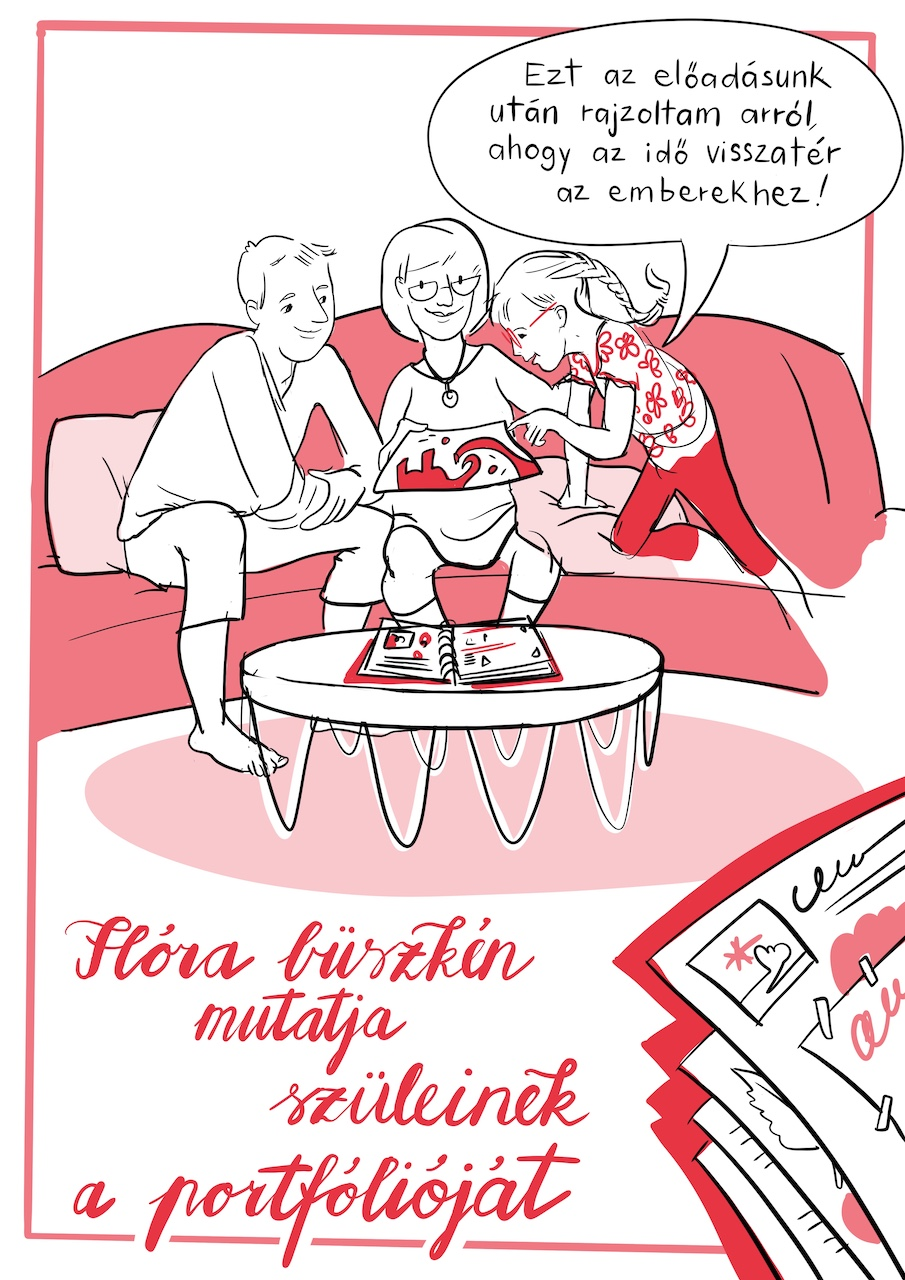
\includegraphics{pics/4b_portfolio_flora.jpg}
\caption{A portfólió segíti, hogy a szülők is jobban tudják követni a gyerekük tanulását, fejlődését. }
\end{figure}

\hypertarget{formai-kovetelmenyek}{%
\paragraph{Formai követelmények}\label{formai-kovetelmenyek}}

A portfóliónak rendezettnek, hozzáférhetőnek, elérhetőnek,
visszakereshetőnek és könnyen bővíthetőnek kell lennie.
A tanulóközösségeknek 
olyan
(technológiai) megoldást kell választaniuk,\break
aminek
alapján a gyerek, tanár és a szülő \emph{naponta} tudja a portfóliót
bővíteni, és akár \emph{heti rendszerességgel} át tudják tekinteni
időrendben, modulonként vagy tantárgyanként a portfólió bővülését.
